% ***************************************************************************************************
%
%	Szablon pracy magisterskiej dla Politechniki Wrocławskiej w wersji dwustronnej.
%	Autor:	Tomasz Strzałka
%
% ***************************************************************************************************

% Styl dwustronny z domyślną wielkością czcionki 10pt oraz oddzieloną stroną tytułową (titlepage).
% Domyślnie rodziały rozpoczynają się na stronie prawej (openright).
\documentclass{book}

% ***************************************************************************************************
% Ustawienia języka
% ***************************************************************************************************

% Podstawowe ustawienia języka, według którego formatowany będzie dokument
\usepackage[polish]{babel}

% Pakiet babel dla polskiego języka powoduje konflikt z pakietem amssymb.
% Polecenie '\lll' definiują oba pakiety - porządana jest druga definicja.
\let\lll\undefined

% W przypadku wielojęzykowości ustawia główny język dokumentu
\selectlanguage{polish}

% Kodowanie dokumentu
\usepackage[utf8]{inputenc}

% Dowolny rozmiar czcionek, kodowanie znaków
\usepackage{lmodern}

% Polskie wcięcia akapitów
\usepackage{indentfirst}

% Polskie łamanie wyrazów
\usepackage[plmath]{polski}

% Przecinek w wyrażeniach matematycznych zamiast kropki
\usepackage{icomma}

% Polskie formatowanie typograficzne
\frenchspacing

% Zapewnia liczne usprawnienia wyświetlania i organizacji matematycznych formuł. 
\usepackage{amsmath}

% Wprowadza rozszerzony zestaw symboli m.in. \leadsto
\usepackage{amssymb}

% Dodatkowa, ,,kręcona'' czcionka matematyczna
\usepackage{mathrsfs}

% Dodatkowe wsparcie dla środowiska mathbb, które nie wspiera domyślnie cyfr (\mathbb{})
\usepackage{bbold}

% Fixes/improves amsmath
\usepackage{mathtools}


% ***************************************************************************************************
% Kolory  
% ***************************************************************************************************

% Umożliwia kolorowanie poszczególnych komórek tabeli
\usepackage[table]{xcolor}% http://ctan.org/pkg/

% Umożliwia łatwą zmianę koloru linii w tabeli
\usepackage{tabu}

% Umożliwia rozszerzoną kontrolę nad kolorami.
\usepackage{xcolor}

% Definicje kolorów
\definecolor{lgray}{HTML}{9F9F9F}
\definecolor{dgray}{HTML}{5F5F5F}
% lgray				-	nazwa nowo zdefiniowanego koloru
% HTML				-	model kolorów
% CCCCCC			-	wartość koloru zgodna z modelem

% ***************************************************************************************************
% Algorytmy 
% ***************************************************************************************************

% Udostępnia środowisko do konstruowania pseudokodów
\usepackage[ruled,vlined,linesnumbered,longend,algochapter]{algorithm2e}
% ruled	- poziome kreski na początku i końcu algorytmu, podpis na górze oddzielony również kreską poziomą
% vlined - pionowe kreski łączące początek polecenia z jego końcem
% linesnumbered	- numerowanie kolejnych wierszy algorytmu
% longend - długie końcówki np. ifend, forend itd.
% algochapter - numeracja z rozdziałami

% Zamiana nazwy środowiska z domyślnej "Algorithm X" na "Pseudokod X"
\newenvironment{pseudokod}[1][htb]{
	\renewcommand{\algorithmcfname}{Pseudokod}
	\begin{algorithm}[#1]%
	}{
\end{algorithm}
}

% Zmiana rozmiaru komentarzy
\newcommand\algcomment[1]{
	\footnotesize{#1}
}

% Ustawienie zadanego stylu dla komentarzy
\SetCommentSty{algcomment}

% Wyśrodkowana tylda
\usepackage{textcomp}%
\newcommand{\textapprox}{\raisebox{0.5ex}{\texttildelow}}

% Listowanie kodów źródłowych
\usepackage{listings} 
\renewcommand{\lstlistingname}{Kod źródłowy} % Polska nazwa listingu

% Definicje pecjalnych znaków, które nie są obsługiwane w środowisku listing
\lstset{literate=
	{ż}{{\.{z}}}1	{ź}{{\'{z}}}1
	{ć}{{\'{c}}}1	{ń}{{\'{n}}}1
	{ą}{{\c a}}1	{ś}{{\'{s}}}1
	{ł}{{\l}}1		{ę}{{\c{e}}}1
	{ó}{{\'{o}}}1	{á}{{\'a}}1
	{é}{{\'e}}1		{í}{{\'i}}1
	{ó}{{\'o}}1		{ú}{{\'u}}1
	{ù}{{\`u}}1		{Á}{{\'A}}1
	{É}{{\'E}}1		{Í}{{\'I}}1
	{Ó}{{\'O}}1		{Ú}{{\'U}}1
	{à}{{\`a}}1		{è}{{\'e}}1
	{ì}{{\`i}}1		{ò}{{\`o}}1
	{ò}{{\`o}}1		{À}{{\`A}}1
	{È}{{\'E}}1		{Ì}{{\`I}}1
	{Ò}{{\`O}}1		{Ò}{{\`O}}1
	{ä}{{\"a}}1		{ë}{{\"e}}1
	{ï}{{\"i}}1		{ö}{{\"o}}1
	{ü}{{\"u}}1		{Ä}{{\"A}}1
	{Ë}{{\"E}}1		{Ï}{{\"I}}1
	{Ö}{{\"O}}1		{Ü}{{\"U}}1
	{â}{{\^a}}1		{ê}{{\^e}}1
	{î}{{\^i}}1		{ô}{{\^o}}1
	{û}{{\^u}}1		{Â}{{\^A}}1
	{Ê}{{\^E}}1		{Î}{{\^I}}1
	{Ô}{{\^O}}1		{Û}{{\^U}}1
	{œ}{{\oe}}1		{Œ}{{\OE}}1
	{æ}{{\ae}}1		{Æ}{{\AE}}1
	{ß}{{\ss}}1		{ç}{{\c c}}1
	{Ç}{{\c C}}1	{ø}{{\o}}1
	{å}{{\r a}}1	{Å}{{\r A}}1
	{€}{{\EUR}}1	{£}{{\pounds}}1
}

% ***************************************************************************************************
% Marginesy 
% ***************************************************************************************************

% Ustawienia rozmiarów stron i ich marginesów
\usepackage[headheight=18pt, top=25mm, bottom=25mm, left=25mm, right=25mm]{geometry}
% headheight		-	wysokość tytułów
% top				-	margines górny
% bottom			-	margines dolny
% left				-	margines lewy
% right				-	margines prawy

% Usunięcie górnego marginesu dla środowisk
\makeatletter
\setlength\@fptop{0\p@}	
\makeatother

% ***************************************************************************************************
% Styl 
% ***************************************************************************************************

% Definiuje środowisko 'titlingpage', które zapewnia pełną kontrolę nad układem strony tytułowej.
\usepackage{titling}


% Umożliwia modyfikowanie stylu spisu treści
\usepackage{tocloft}	

\tocloftpagestyle{tableOfContentStyle}

% Definiowanie własnych stylów nagłówków i/lub stopek
\usepackage{fancyhdr}

% Domyślny styl dla pracy 
\fancypagestyle{custom}{
	\fancyhf{}									% wyczyść stopki i nagłówki
	\fancyhead[RO]{								% Prawy, nieparzysty nagłówek
		\hrulefill \hspace{16pt} \large Rozdział \thechapter
		\put(-472.1, 12.1){%
			\makebox(0,0)[l]{%
				
\includegraphics[width=0.05\textwidth]{pwr-logo}
			}
		}
		\put(-443,5.5){%
			\makebox(0,0)[l]{%
				\small Politechnika Wrocławska
			}
		}
	}
	\fancyhead[LE]{								% Lewy, parzysty nagłówek
		\large Rozdział \thechapter \hspace{16pt} \hrulefill 
		\put(-22, 12.1){%
			\makebox(0,0)[l]{%
				
\includegraphics[width=0.05\textwidth]{wppt-logo}
			}
		}
		\put(-210,5.5){%
			\makebox(0,0)[l]{%
				\small Wydział Podstawowych Problemów Techniki
			}
		}
	}
	\fancyfoot[LE,RO]{							% Stopki
		\thepage
	}
	\renewcommand{\headrulewidth}{0pt}			% Grubość linii w nagłówku
	\renewcommand{\footrulewidth}{0.2pt}		% Grubość linii w stopce
}


% Domyślny styl dla bibliografii
\fancypagestyle{bibliographyStyle}{
	\fancyhf{}									% wyczyść stopki i nagłówki
	\fancyhead[RO]{								% Prawy, nieparzysty nagłówek
		\hrulefill \hspace{16pt} \large Dodatek \thechapter
		\put(-472.1, 12.1){%
			\makebox(0,0)[l]{%
				
\includegraphics[width=0.05\textwidth]{pwr-logo}
			}
		}
		\put(-443,5.5){%
			\makebox(0,0)[l]{%
				\small Politechnika Wrocławska
			}
		}
	}
	\fancyhead[LE]{								% Lewy, parzysty nagłówek
		\large Bibliografia \hspace{16pt} \hrulefill 
		\put(-22, 12.1){%
			\makebox(0,0)[l]{%
				
\includegraphics[width=0.05\textwidth]{wppt-logo}
			}
		}
		\put(-210,5.5){%
			\makebox(0,0)[l]{%
				\small Wydział Podstawowych Problemów Techniki
			}
		}
	}
	\fancyfoot[LE,RO]{							% Stopki
		\thepage
	}
	\renewcommand{\headrulewidth}{0pt}			% Grubość linii w nagłówku
	\renewcommand{\footrulewidth}{0.2pt}		% Grubość linii w stopce
}

% Domyślny styl dla dodatków
\fancypagestyle{appendixStyle}{
	\fancyhf{}									% wyczyść stopki i nagłówki
	\fancyhead[RO]{								% Prawy, nieparzysty nagłówek
		\hrulefill \hspace{16pt} \large Dodatek \thechapter
		\put(-472.1, 12.1){%
			\makebox(0,0)[l]{%
				
\includegraphics[width=0.05\textwidth]{pwr-logo}
			}
		}
		\put(-443,5.5){%
			\makebox(0,0)[l]{%
				\small Politechnika Wrocławska
			}
		}
	}
	\fancyhead[LE]{								% Lewy, parzysty nagłówek
		\large Dodatek \thechapter \hspace{16pt} \hrulefill 
		\put(-22, 12.1){%
			\makebox(0,0)[l]{%
				
\includegraphics[width=0.05\textwidth]{wppt-logo}
			}
		}
		\put(-210,5.5){%
			\makebox(0,0)[l]{%
				\small Wydział Podstawowych Problemów Techniki
			}
		}
	}
	\fancyfoot[LE,RO]{							% Stopki
		\thepage
	}
	\renewcommand{\headrulewidth}{0pt}			% Grubość linii w nagłówku
	\renewcommand{\footrulewidth}{0.2pt}		% Grubość linii w stopce
}

% Osobny styl dla stron zaczynających rozdział/spis treści itd. (domyślnie formatowane jako "plain")
\fancypagestyle{chapterBeginStyle}{
	\fancyhf{}%
	\fancyfoot[LE,RO]{
		\thepage
	}
	\renewcommand{\headrulewidth}{0pt}
	\renewcommand{\footrulewidth}{0.2pt}
}

% Styl dla pozostałych stron spisu treści
\fancypagestyle{tableOfContentStyle}{
	\fancyhf{}%
	\fancyfoot[LE,RO]{
		\thepage
	}
	\renewcommand{\headrulewidth}{0pt}
	\renewcommand{\footrulewidth}{0.2pt}
}

% Formatowanie tytułów rozdziałów i/lub sekcji
\usepackage{titlesec}

% Formatowanie tytułów rozdziałów
\titleformat{\chapter}[hang]					% kształt
{
	\vspace{-10ex}
	\Huge
	\bfseries
}												% formatowanie tekstu modyfikowanego elementu
{}												% etykieta występująca przed tekstem modyfikowanego elementu, niewidoczna w spisie treści
{
	10pt
}												% odstęp formatowanego tytułu od lewego marginesu/etykiety
{
	\Huge
	\bfseries
}												% formatowanie elementów przed modyfikowanym tytułem
[
\vspace{2ex}
%\rule{\textwidth}{0.4pt}
%\vspace{-4ex}
]												% dodatkowe formatowanie stosowane poniżej modyfikowanego tytułu


% Formatowanie tytułów sekcji
\titleformat{\section}[hang]					% kształt
{
	\vspace{2ex}
%	\titlerule\vspace{1ex}
	\Large\bfseries
}												% formatowanie tekstu modyfikowanego elementu
{
	\thesection									% etykieta występująca przed tekstem modyfikowanego elementu, niewidoczna w spisie treści
}
{
	0pt
}												% odstęp formatowanego tytułu od lewego marginesu/etykiety
{
	\Large
	\bfseries
}												% formatowanie elementów przed modyfikowanym tytułem

% ***************************************************************************************************
% Linki
% ***************************************************************************************************

% Umożliwia wstawianie hiperłączy do dokumentu
\usepackage{hyperref}							% Aktywuje linki

\hypersetup{
	colorlinks	=	true,					% Koloruje tekst zamiast tworzyć ramki.
	linkcolor		=	blue,					% Kolory: referencji,
        citecolor		=	blue,					% cytowań,
	urlcolor		=	blue					% hiperlinków.
}

% Do stworzenia hiperłączy zostanie użyta ta sama (same) czcionka co dla reszty dokumentu
\urlstyle{same}




% ***************************************************************************************************
% Linki
% ***************************************************************************************************

% Umożliwia zdefiniowanie własnego stylu wyliczeniowego
\usepackage{enumitem}

% Nowa lista numerowana z trzema poziomami
\newlist{myitemize}{itemize}{3}

% Definicja wyglądu znacznika pierwszego poziomu
\setlist[myitemize,1]{
	label		=	\textbullet,
	leftmargin	=	4mm}

% Definicja wyglądu znacznika drugiego poziomu
\setlist[myitemize,2]{
	label		=	$\diamond$,
	leftmargin	=	8mm}

% Definicja wyglądu znacznika trzeciego poziomu
\setlist[myitemize,3]{
	label		=	$\diamond$,
	leftmargin	=	12mm
}

% ***************************************************************************************************
% Inne pakiety
% ***************************************************************************************************

% Dołączanie rysunków
\usepackage{graphicx}

% Figury i przypisy
\usepackage{caption}
\usepackage{subcaption}

% Umożliwia tworzenie przypisów wewnątrz środowisk
\usepackage{footnote}

% Umożliwia tworzenie struktur katalogów
\usepackage{dirtree}

% Rozciąganie komórek tabeli na wiele wierszy
\usepackage{multirow}

% Precyzyjne obliczenia szerokości/wysokości dowolnego fragmentu wygenerowanego przez LaTeX
\usepackage{calc}

% ***************************************************************************************************
% Matematyczne skróty
% ***************************************************************************************************

% Skrócony symbol liczb rzeczywistych
\newcommand{\RR}{\mathbb{R}}

% Skrócony symbol liczb naturalnych
\newcommand{\NN}{\mathbb{N}}

% Skrócony symbol liczb wymiernych
\newcommand{\QQ}{\mathbb{Q}}

% Skrócony symbol liczb całkowitych
\newcommand{\ZZ}{\mathbb{Z}}

% Skrócony symbol logicznej implikacji
\newcommand{\IMP}{\rightarrow}

% Skrócony symbol  logicznej równoważności
\newcommand{\IFF}{\leftrightarrow}

% ***************************************************************************************************
% Środowiska
% ***************************************************************************************************

% Środowisko do twierdzeń
\newtheorem{theorem}{Twierdzenie}[chapter]

% Środowisko do lematów
\newtheorem{lemma}{Lemat}[chapter]

% Środowisko do przykładów
\newtheorem{example}{Przykład}[chapter]

% Środowisko do wniosków
\newtheorem{corollary}{Wniosek}[chapter]

% Środowisko do definicji
\newtheorem{definition}{Definicja}[chapter]

% Środowisko do dowodów
\newenvironment{proof}{
	\par\noindent \textbf{Dowód.}
}{
\begin{flushright}
	\vspace*{-6mm}\mbox{$\blacklozenge$}
\end{flushright}
}

% Środowisko do uwag
\newenvironment{remark}{
	\bigskip \par\noindent \small \textbf{Uwaga.}
}{
\begin{small}
	\vspace*{4mm}
\end{small}
}

% ***************************************************************************************************
% Słownik
% ***************************************************************************************************

% Prawidłowe dzielenie wyrazów
\hyphenation{wszy-stkich ko-lu-mnę każ-da od-leg-łość
	dzie-dzi-ny dzie-dzi-na rów-nych rów-ny
	pole-ga zmie-nna pa-ra-met-rów wzo-rem po-cho-dzi
	o-trzy-ma wte-dy wa-run-ko-wych lo-gicz-nie
	skreś-la-na skreś-la-ną cał-ko-wi-tych wzo-rów po-rzą-dek po-rząd-kiem
	przy-kład pod-zbio-rów po-mię-dzy re-pre-zen-to-wa-ne
	rów-no-waż-ne bi-blio-te-kach wy-pro-wa-dza ma-te-ria-łów
	prze-ka-za-nym skoń-czo-nym moż-esz na-tu-ral-na cią-gu tab-li-cy
	prze-ka-za-nej od-po-wied-nio}

% ***************************************************************************************************
% Dokument
% ***************************************************************************************************

\frontmatter

\begin{document}

	\begin{titlingpage}
		\vspace*{\fill}
		\begin{center}
			\begin{picture}(300,510)
				\put(11,520){\makebox(0,0)[l]{\large \textsc{Wydział Podstawowych Problemów Techniki}}}
				\put(11,500){\makebox(0,0)[l]{\large \textsc{Politechnika Wrocławska}}}
% Tytuł pracy
				\put(80,320){\Huge \textsc{Implementacja}}
				\put(80,280){\Huge \textsc{abstrakcyjnej}}
				\put(80,240){\Huge \textsc{maszyny Warrena}}
% Autor pracy
				\put(90,200){\makebox(0,0)[l]{\large \textsc{Kajetan Bilski}}}
				\put(90,180){\makebox(0,0)[l]{\large \textsc{Nr indeksu: 244942}}}

				\put(200,100){\makebox(0,0)[l]{\large Praca inżynierska napisana}}
				\put(200,80){\makebox(0,0)[l]{\large pod kierunkiem}}
% dane promotora
				\put(200,60){\makebox(0,0)[l]{\large Dr Przemysława Kobylańskiego}}
				
				\put(115,-70){
\includegraphics[width=0.15\textwidth]{pwr}}
				\put(106,-80){\makebox(0,0)[bl]{\large \textsc{Wrocław 2020}}}
			\end{picture}
		\end{center}	
		\vspace*{\fill}
	\end{titlingpage}
	
        \cleardoublepage
		
	\pagenumbering{Roman}
	\pagestyle{tableOfContentStyle}
	\tableofcontents
	\cleardoublepage
		
	% ***************************************************************************************************
	% Wstęp
	% ***************************************************************************************************
	
	\pagestyle{custom}
	\mainmatter
	
	% ***************************************************************************************************
	% Rodziały
	% ***************************************************************************************************

	\chapter{Wstęp}
\thispagestyle{chapterBeginStyle}

\iffalse
Praca dyplomowa inżynierska jest dokumentem opisującym zrealizowany system techniczny. Praca powinna być napisana poprawnym językiem odzwierciedlającym aspekty techniczne (informatyczne) omawianego zagadnienia. Praca powinna być napisana w trybie bezosobowym (w szczególności należy unikać trybu pierwszej osoby liczby pojedynczej i mnogiej). Zdania opisujące konstrukcję systemu informatycznego powinny być tworzone w stronie biernej. W poniższym dokumencie przykłady sformułowań oznaczono kolorem niebieskim. W opisie elementów systemu, komponentów, elementów kodów źródłowych, nazw plików, wejść i wyjść konsoli należy stosować czcionkę stałej szerokości, np: {\color{lgray}zmienna \verb|wynik| przyjmuje wartość zwracaną przez funkcję \verb|dodaj(a,b)|, dla argumentów \verb|a| oraz \verb|b| przekazywanych \ldots}.

Układ poniższego dokumentu przedstawia wymaganą strukturę pracy, z rozdziałami zawierającymi analizę zagadnienia, opis projektu systemu oraz implementację (dobór podrozdziałów jest przykładowy i należy go dostosować do własnej tematyki pracy). 
  
Wstęp pracy (nie numerowany) powinien składać się z czterech części (które nie są wydzielane jako osobne podrozdziały): zakresu pracy, celu, analizy i porównania istniejących rozwiązań oraz przeglądu literatury, oraz opisu zawartości pracy.

Każdy rozdział powinien rozpoczynać się od akapitu wprowadzającego, w którym zostaje w skrócie omówiona zawartość tego rozdziału.

{\color{dgray}
Praca swoim zakresem obejmuje wielowarstwowe rozproszone systemy informatyczne typu ,,B2B'' wspierające wymianę danych pomiędzy przedsiębiorstwami. Systemy tego typu, konstruowane dla dużych korporacji, charakteryzują się złożoną strukturą poziomą i pionową, w której dokumenty \ldots

Celem pracy jest zaprojektowanie i oprogramowanie aplikacji o następujących założeniach funkcjonalnych:
\begin{itemize}
    \item wspieranie zarządzania obiegiem dokumentów wewnątrz korporacji z uwzględnieniem \ldots,
	\item wspieranie zarządzania zasobami ludzkimi z uwzględnieniem modułów kadrowych oraz \ldots,
	\item gotowość do uzyskania certyfikatu ISO \ldots,
	\item \ldots.
\end{itemize}

Istnieje szereg aplikacji o zbliżonej funkcjonalności: \ldots, przy czym \ldots.

Praca składa się z czterech rozdziałów.
W rozdziale pierwszym omówiono strukturę przedsiębiorstwa \ldots, scharakteryzowano grupy użytkowników oraz przedstawiono procedury związane z obiegiem dokumentów. Szczegółowo opisano mechanizmy \ldots. Przedstawiono uwarunkowania prawne udostępniania informacji \ldots, w ramach \ldots.

W rozdziale drugim przedstawiono szczegółowy projekt systemy w notacji UML. Wykorzystano diagramy \ldots.
Opisano w pseudokodzie i omówiono algorytmy generowania \ldots.

W rozdziale trzecim opisano technologie implementacji projektu: wybrany język programowania, biblioteki, system zarządzania bazą danych, itp.  Przedstawiono dokumentację techniczną kodów źródłowych interfejsów poszczególnych modułów systemu. Przedstawiono sygnatury metod publicznych oraz \ldots.

W rozdziale czwartym przedstawiono sposób instalacji i wdrożenia systemu w środowisku docelowym.

Końcowy rozdział stanowi podsumowanie uzyskanych wyników.
}
\fi


Celem pracy było zaimplementowanie abstrakcyjnej maszyny Warrena dla czystego języka Prolog. Odpowiada on językowi trzeciego poziomu z opisu maszyny. Praca zawiera, poza opisem implementacji, analizę efektywności jej działania na wybranych przykładach programów.
Oprócz tego praca zawiera kompilator służący do kompilacji czystego języka Prolog na instrukcje maszyny Warrena.\\
W wielu językach programowania, np. C/C++, kompilator zamienia kod języka na kod maszynowy, który może być wykonany przez system operacyjny. Prolog różni się pod tym względem, ponieważ jego skompilowany kod nie jest wykonywany przez system operacyjny, a przez maszynę Warrena (WAM). Prolog jest językiem programowania logicznego i jego działanie opiera się na udowodnieniu zapytania zadanego przez programistę za pomocą faktów i reguł (wbudowanych lub również danych przez programistę) i zwraca wynik oznaczający prawdziwość zapytania (czy da się je udowodnić). Prolog próbuje udowodnić zapytanie na wszystkie dostępne sposoby, które umożliwiają dane predykaty. Implementacja abstrakcyjnej maszyny Warrena musi zawierać całą tą funkcjonalność. Moja implementacja dla większej łatwości użytkowania i lepszego porównania z innymi implementacjami zawiera wbudowany kompilator, który w pojedynczym uruchomieniu może być używany razem z maszyną, ale może być też uruchomiony osobno. Oprócz tego sama maszyna zawiera wbudowane predykaty i instrukcje, które nie są częścią czystego Prologa, ale dają lepszy wgląd w jej działanie.
	\cleardoublepage

	\chapter{Wykorzystane technologie i instrukcja obsługi}
\thispagestyle{chapterBeginStyle}

\iffalse
W tym rozdziale należy przedstawić analizę zagadnienia, które podlega informatyzacji. Należy zidentyfikować i opisać obiekty składowe rozważanego wycinka rzeczywistości i ich wzajemne relacje (np.\ użytkowników systemu i ich role). Należy szczegółowo omówić procesy jakie zachodzą w systemie i które będą informatyzowane, takie jak np.\ przepływ dokumentów.
Należy sprecyzować i wypunktować założenia funkcjonalne i poza funkcjonalne dla projektowanego systemu.
Jeśli istnieją aplikacje realizujące dowolny podzbiór zadanych funkcjonalności realizowanego systemu należy przeprowadzić ich analizę porównawczą, wskazując na różnice bądź innowacyjne elementy, które projektowany w pracy system informatyczny będzie zawierał.
Należy odnieść się do uwarunkowań prawnych związanych z procesami przetwarzania danych w projektowanym systemie.
Jeśli zachodzi konieczność, należy wprowadzić i omówić model matematyczny elementów systemu na odpowiednim poziomie abstrakcji.

{\color{dgray}
W niniejszym rozdziale omówiono koncepcję architektury programowej systemu \ldots. W
szczególny sposób \ldots. Omówiono założenia funkcjonalne i niefunkcjonalne podsystemów \ldots. Przedstawiono
mechanizmy \ldots. Sklasyfikowano systemy ze względu na \ldots. Omówiono istniejące rozwiązania informatyczne o podobnej funkcjonalności \ldots (zobacz \cite{JCINodesChord}).
}
\fi

Program działa w terminalu na linuksie (był testowany na Ubuntu w WSL). Do jego kompilacji zostały użyte: g++ 7.5.0, flex 2.6.4, GNU Bison 3.0.4 i GNU Make 4.1. WAM został napisany w C++ w standardzie C++14.\\

Sposoby użycia:\\
\texttt{wam [<program>]}\\
\texttt{wam -c <input> [<output>]}\\
\texttt{wam -e <program> <query>}\\

W pierwszym przypadku użycia \texttt{program} jest ścieżką do pliku z programem napisanym w języku Prolog. Program jest ładowany do pamięci, następnie WAM wyświtla "?-" i czeka na użytkownika, żeby wpisał zapytanie. Zapytanie musi być w jednej linii i kończyć się kropką. Po wykonaniu zapytania WAM resetuje swoją pamięć i oczekuje następnego zapytania od użytkownika i tak dalej w pętli aż użytkownik nie wyjdzię manualnie (ctrl+C).\\
W drugim przypadku użycia pobiera z pliku tektowego \texttt{input} program lub zapytanie i kompiluje go do listy instrukcji maszyny Warrena, które umieszcze w pliku tekstowym \texttt{output} jeśli został podany lub w \texttt{a.out} w przeciwnym wypadku. Kompilator rozróżnia program i zapytanie Prologa po tym, że zapytanie musi rozpoczynać się od "?-".\\
W trzecim przypadku użycia \texttt{program} i \texttt{query} są plikami tekstowymi zawierającymi instrukcje maszyny Warrena, takimi jakie można wygenerować używając opcji \texttt{-c}. WAM ładuje wykonuje te instrukcje pomijając kompilator.\\

	\cleardoublepage

	\chapter{WAM - Abstrakcyjna maszyna Warrena}
\thispagestyle{chapterBeginStyle}

\iffalse
W tym rozdziale należy przedstawić analizę zagadnienia, które podlega informatyzacji. Należy zidentyfikować i opisać obiekty składowe rozważanego wycinka rzeczywistości i ich wzajemne relacje (np.\ użytkowników systemu i ich role). Należy szczegółowo omówić procesy jakie zachodzą w systemie i które będą informatyzowane, takie jak np.\ przepływ dokumentów.
Należy sprecyzować i wypunktować założenia funkcjonalne i poza funkcjonalne dla projektowanego systemu.
Jeśli istnieją aplikacje realizujące dowolny podzbiór zadanych funkcjonalności realizowanego systemu należy przeprowadzić ich analizę porównawczą, wskazując na różnice bądź innowacyjne elementy, które projektowany w pracy system informatyczny będzie zawierał.
Należy odnieść się do uwarunkowań prawnych związanych z procesami przetwarzania danych w projektowanym systemie.
Jeśli zachodzi konieczność, należy wprowadzić i omówić model matematyczny elementów systemu na odpowiednim poziomie abstrakcji.

{\color{dgray}
W niniejszym rozdziale omówiono koncepcję architektury programowej systemu \ldots. W
szczególny sposób \ldots. Omówiono założenia funkcjonalne i niefunkcjonalne podsystemów \ldots. Przedstawiono
mechanizmy \ldots. Sklasyfikowano systemy ze względu na \ldots. Omówiono istniejące rozwiązania informatyczne o podobnej funkcjonalności \ldots (zobacz \cite{JCINodesChord}).
}
\fi

W tym rozdziale opiszę technologie (np. wersję kompilatora) i sposób użycia programu będącego maszyną.
	\cleardoublepage

	\chapter{Struktura pamięci}
\thispagestyle{chapterBeginStyle}

\iffalse
{\color{dgray}
W tym rozdziale przedstawiono szczegółowy projekt systemy w notacji UML uwzględniający wymagania funkcjonalne opisane w rozdziale~\ref{rozdzial1}. Do opisu relacji pomiędzy składowymi systemu wykorzystano diagramy \ldots.
Przedstawiono w pseudokodzie i omówiono algorytmy generowania \ldots.
}


\section{Grupy użytkowników i założenia}

{\color{dgray}
Architektura systemu \ldots jest wielowarstwowa i rozproszona, przy czym \ldots. Podsystem  \ldots jest systemem zbiorczym dla danych \ldots wysyłanych do serwera \ldots. 

Taka architektura jest zgodna z wzorcem projektowym MVC\footnote{Należy odnieść się do wykorzystywanych wzorców projektowych} (ang.  Model-View-Controller). Przetwarzanie danych odbywa się \ldots.
} 

\section{Przypadki użycia i scenariusze}

W tej sekcji należy przedstawić przypadki użycia oraz odpowiadające im scenariusze dla poszczególnych grup użytkowników \ldots.

\section{Diagramy klas}

W tej sekcji należy przedstawić diagramy klas dla odpowiednich elementów systemu zidentyfikowane na podstawie wcześniejszych rozważań 

\section{Diagramy aktywności}

W tej sekcji należy przedstawić diagramy aktywności dla elementów systemu i odpowiednich procesów wynikające z wcześniejszej analizy.  

{\color{dgray}
W niniejszym rozdziale przedstawiono diagramy aktywności \ldots. Diagram na rysunku~\ref{czynnosci_GD} przedstawia \ldots.
} 

\begin{figure}[h!]
\begin{center}
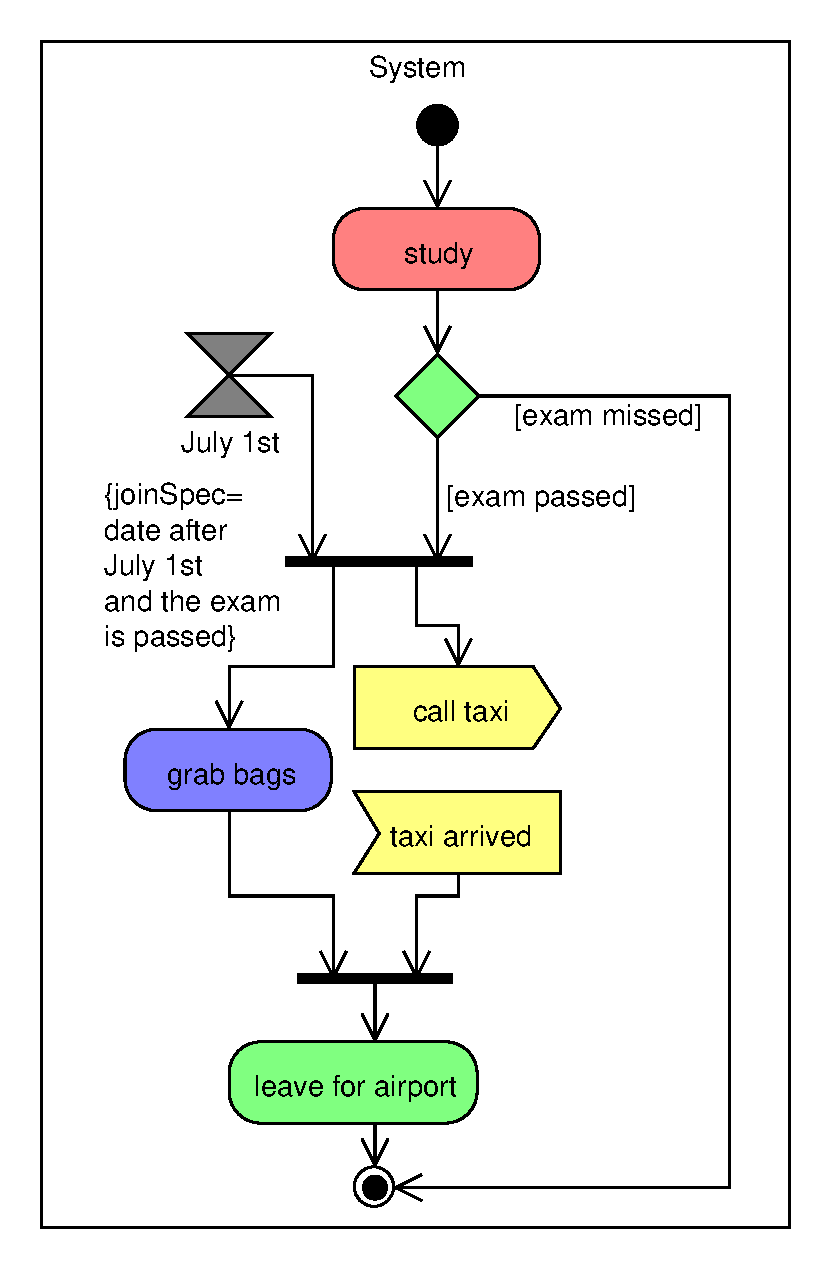
\includegraphics[width=0.5\textwidth]{aktyw.pdf}
\end{center}
\caption{{\color{dgray}Diagram aktywności związany z procesem rejestracji dokumentu.}} \label{czynnosci_GD}
\end{figure}  

\section{Diagramy sekwencji}

W tej sekcji należy przedstawić diagramy sekwencji dla obiektów systemu zidentyfikowanych na podstawie wcześniejszych rozważań. Należy wykorzystać nazewnictwo wprowadzone w poprzednich rozdziałach, w szczególności odpowiadające definicjom wprowadzonych klas.

\section{Diagramy stanów}

W tej sekcji należy przedstawić diagramy stanów w których może znaleźć się system. Diagramy te są szczególnie istotne przy projektowaniu systemów czasu rzeczywistego. 

\section{Projekt bazy danych}

W tej sekcji należy przedstawić projekt bazy danych. Należy omówić wycinek rzeczywistości i odpowiadające mu zidentyfikowane elementy systemu, których wartości będą podlegać utrwalaniu. Należy przedyskutować wybór typów danych dla atrybutów poszczególnych obiektów. Należy uzasadnić wybór platformy DBMS. Dla relacyjnych baz danych należy przedyskutować jej normalizację.

\section{Opis protokołów}

W tej sekcji należy omówić protokoły wykorzystywane przez komponenty systemu. Omówić formaty komunikatów i zilustrować je przykładami. 

\section{Opis algorytmów}

W tej sekcji należy wymienić i przedyskutować algorytmy wykorzystywane w systemie. Algorytmy należy przedstawić w pseudokodzie (wykorzystać pakiet \texttt{algorithm2e}). Omówienia poszczególnych kroków algorytmów powinny zawierać odwołania do odpowiednich linii pseudokodu. Dla zaproponowanych autorskich algorytmów należy przeprowadzić analizę ich złożoności czasowej i pamięciowej. 

{\color{dgray}
Algorytm bąblowania jest przedstawiony w Pseudokodzie~\ref{alg:mine}.
}

{\small
\begin{pseudokod}[H]
%\SetAlTitleFnt{small}
\SetArgSty{normalfont}
\SetKwFunction{Process}{Process}
\SetKwFunction{Calculate}{Calculate}
\KwIn{Zbiór bąbli $B$}
\KwOut{Wyporność $W$}
\ForEach{$b \in B$}{
\Process{$b$}\;
\For{$i \leftarrow 1$ \KwTo $|B|$}{
\If{\Calculate{EW($i$,$b$)} $\le$ 0}{
$b \leftarrow 2*b$\;
}
}
}
\While{$B \neq \emptyset$}{
\For{$j \leftarrow 1$ \KwTo $|B|$}{
\If{\Calculate{FT($j$,$\hat{b}$)} $\le 0$}{
$w \leftarrow 2*\hat{b}$\;
$W \leftarrow W \cup \{w\}$\;
$B \leftarrow B \setminus \{b\}$\;
}
}
}
\caption{Wyporność przez bąblowanie}\label{alg:mine}
\end{pseudokod}
}
\fi

W tym rozdziale opiszę jak działa pamięć maszyny. Wszystkie zmienne reprezentujące elementy pamięci maszyny są zmiennymi globalnymi.

\section{Komórka pamięci}

Komórka pamięci to podstawowa składowa wielu elementów pamięci. Każda komórka ma jeden z dwóch typów. Komórka zmiennej zawiera tag, który może być {REF} lub {STR}, a także adres dowolnej innej komórki znajdującej się w pamięci. Komórka funktora zawiera reprezentację funktora $f/n$, gdzie $f$ jest nazwą funktora, a $n$ liczbą argumentów przez niego przyjmowanych. Domyślnie każda komórka jest komórką zmiennej o tagu {REF} i adresie pokazującym na samą siebie.

\section{{HEAP} - Sterta}

\section{Rejestry tymczasowe}

\section{Rejestry trwałe}

\section{{CODE} - Magazyn kodu}

\section{{P} i {CP}}

\section{{STACK} - Stos}


	\cleardoublepage
	
	\chapter{Instrukcje Maszyny}
\thispagestyle{chapterBeginStyle}

\iffalse
\section{Opis technologii}

Należy tutaj zamieścić krótki opis (z referencjami) do technologii użytych przy implementacji systemu.

{\color{dgray}
Do implementacji systemu użyto języka JAVA w wersji \ldots, szczegółowy opis można znaleźć w \cite{Java}. Interfejs zaprojektowano w oparciu o HTML5 i CSS3 \cite{HTML-CSS}.
}

\section{Omówienie kodów źródłowych}

{\color{dgray}
Kod źródłowy~\ref{ws} przedstawia opisy poszczególnych metod interfejsu: \texttt{WSPodmiotRejestracjaIF}. Kompletne
kody źródłowe znajdują się na płycie CD dołączonej do niniejszej pracy w katalogu \texttt{Kody} (patrz Dodatek~\ref{plytaCD}).
}

\begin{small}
\begin{lstlisting}[language=Java, frame=lines, numberstyle=\tiny, stepnumber=5, caption=Interfejs usługi Web Service: \texttt{WSPodmiotRejestracjaIF}\label{ws}., firstnumber=1]
package erejestracja.podmiot;
import java.rmi.RemoteException;
// Interfejs web serwisu dotyczącego obsługi podmiotów i rejestracji.
public interface WSPodmiotRejestracjaIF extends java.rmi.Remote{
// Pokazuje informacje o danym podmiocie.
// parametr: nrPeselRegon - numer PESEL podmiotu lub numer REGON firmy.
// return: Podmiot - obiekt transportowy: informacje o danym podmiocie.
public Podmiot pokazPodmiot(long nrPeselRegon) throws RemoteException;
// Dodaje nowy podmiot.
// parametr: nowyPodmiot - obiekt transportowy: informacje o nowym podmiocie.
// return: true - jeśli podmiot dodano, false - jeśli nie dodano.
public boolean dodajPodmiot(Podmiot nowyPodmiot) throws RemoteException;
// Usuwa dany podmiot.
// parametr: nrPeselRegon - numer PESEL osoby fizycznej lub numer REGON firmy.
// return: true - jeśli podmiot usunięto, false - jeśli nie usunięto.
public boolean usunPodmiot(long nrPeselRegon) throws RemoteException;
// Modyfikuje dany podmiot.
// parametr: podmiot - obiekt transportowy: informacje o modyfikowanym podmiocie.
// return: true - jeśli podmiot zmodyfikowano, false - jeśli nie zmodyfikowano.
public boolean modyfikujPodmiot(Podmiot podmiot) throws RemoteException;
// Pokazuje zarejestrowane podmioty na dany dowód rejestracyjny.
// parametr: nrDowoduRejestracyjnego - numer dowodu rejestracyjnego.
// return: PodmiotRejestracja[] - tablica obiektów transportowych: informacje o
// wszystkich zarejestrowanych podmiotach.
public PodmiotRejestracja[] pokazZarejestrowanePodmioty(
String nrDowoduRejestracyjnego) throws RemoteException;
// Nowa rejestracja podmiotu na dany dowód rejestracyjny.
// parametr: nrDowoduRejestracyjnego - numer dowodu rejestracyjnego.
// parametr: nrPeselRegon - numer PESEL podmiotu lub numer REGON firmy.
// parametr: czyWlasciciel - czy dany podmiot jest właścicielem pojazdu.
// return: true - jeśli zarejestrowano podmiot, false - jeśli nie zarejestrowano.
public boolean zarejestrujNowyPodmiot(String nrDowoduRejestracyjnego,
long nrPeselRegon, boolean czyWlasciciel) throws RemoteException;
// Usuwa wiązanie pomiędzy danym podmiotem, a dowodem rejestracyjnym.
// parametr: nrDowoduRejestracyjnego - numer dowodu rejestracyjnego.
// parametr: nrPeselRegon - numer PESEL podmiotu lub numer REGON firmy.
// return: true - jeśli podmiot wyrejestrowano, false - jeśli nie wyrejestrowano.
public boolean wyrejestrujPodmiot(String nrDowoduRejestracyjnego,
long nrPeselRegon) throws RemoteException;
\end{lstlisting} 
\end{small}

{\color{dgray}
Kod źródłowy~\ref{req} przedstawia procedurę przetwarzającą żądanie. Hasz utrwalany \verb|%granulacja| wykorzystywany jest do komunikacji międzyprocesowej.
}

\begin{small}
\begin{lstlisting}[language=perl, frame=lines, caption=Przetwarzanie żądania - procedura \texttt{process\_req()}\label{req}., firstnumber=86]
sub process_req(){	
  my($r) = @_;
  $wyn = "";
  if ($r=~/get/i) {
	@reqest = split(" ",$r);
	$zad = $reqest[0];
	$ts1 = $reqest[1];
	$ts2 = $reqest[2];
	@date1 = split(/\D/,$ts1);
	@date2 = split(/\D/,$ts2);
	print "odebralem: $r"; 
	$wyn = $wyn."zadanie: $zad\n";
	$wyn = $wyn."czas_od: "."$date1[0]"."-"."$date1[1]"."-"."$date1[2]"."_"."$date1[3]".":"."$date1[4]".":"."$date1[5]"."\n";
	$wyn = $wyn."czas_do: "."$date2[0]"."-"."$date2[1]"."-"."$date2[2]"."_"."$date2[3]".":"."$date2[4]".":"."$date2[5]"."\n";		
	$wyn = $wyn.&sym_sens($ts1,$ts2);
	return $wyn;
  }
  if ($r=~/set gt/i) {
	@reqest = split(" ",$r);
	$zad = $reqest[0];
	$ts1 = $reqest[1];
	$ts2 = $reqest[2];
	$gt = $reqest[2];
	dbmopen(%granulacja,"granulacja_baza",0644);
	$granulacja{"gt"}=$gt;
	dbmclose(%granulacja);
	$wyn = "\'GT\' zmienione na: $gt";
  }		
}	
\end{lstlisting} 
\end{small}
\fi

Główna pętla progarmu polega na wywołaniu instrukcji \texttt{CODE[P]} i zwiększeniu \texttt{P} o 1 do momentu dojścia do końca kodu lub w trakcie wykonywania instrkcji zwrócenia $fail$. W pierwszym wypadku pojawia wykonywanie zapytania kończy się powodzeniem i użytkownik zostaje zapytany czy chce kontynuować. Jeśli wybierze "tak" to program wraca do wykonywania zapytania, tak jakby instrukcja zwróciła $fail$. Jeśli wykowana instrukcja zwróci $fail$, to jeśli jest aktywny punkt wyboru to wyknonywana jest operacja nawrotu i zapytanie wykonywane jest dalej. Jeżeli nie ma aktywnego punktu wyboru, to wykonywanie zapytania kończy się z wynikiem $fałsz$.\\
Poniżej opisane są wszystkie obsługiwane instrukcje.

\section{\texttt{put\_structure} $f/n$,\texttt{X}$i$}

Dodaje na koniec sterty komórkę STR i komórkę funktora $f/n$, której adres zawiera. Następnie kopiuje tą komórkę STR do rejestru o adresie \texttt{X}$i$.

\section{\texttt{set\_variable} \texttt{X}$i$}

Dodaje na koniec sterty nieprzypisaną komórkę REF, a następnie umieszcza w rejestrze \texttt{X}$i$ komórkę REF z jej adresem.

\section{\texttt{set\_value} \texttt{X}$i$}

Dodaje na koniec sterty komórkę będącą kopią komórki z rejestru \texttt{X}$i$.

\section{\texttt{get\_structure} $f/n$,\texttt{X}$i$}

Wywołuje $deref(\texttt{X}i)$ i jeżeli otrzymany adres pokazuje na nieprzypisaną komórkę, to dodaje na koniec sterty komórkę STR i komórkę funktora $f/n$, której adres zawiera. Następnie wywołuje $bind(deref(\texttt{X}i),\texttt{H})$ i ustawia tryb maszyny na $write$ i adres \texttt{S} na koniec sterty. W przeciwnym wypadku jeśli $deref(\texttt{X}i)$ pokazuje na komórkę STR z adresem $addr$, to ustawia \texttt{S} na $addr+1$ i tryb maszyny na $read$.

\section{\texttt{unify\_variable} \texttt{X}$i$}

Jeśli maszyna jest w trybie $read$ to kopiuje komórkę z adresu \texttt{S} do rejestru \texttt{X}$i$.\\
Jeśli maszyna jest w trybie $write$ to dodaje na koniec stery nieprzypisaną komórkę i kopiuje ją do rejestru \texttt{X}$i$.

\section{\texttt{unify\_value} \texttt{X}$i$}

Jeśli maszyna jest w trybie $read$ to wywołuje $unify(\texttt{X}i, \texttt{S})$.\\
Jeśli maszyna jest w trybie $write$ to kopiuje komórkę z rejestru \texttt{X}$i$ na koniec sterty.

\section{\texttt{put\_variable} \texttt{X}$i$ \texttt{A}$j$}

Dodaje na koniec sterty nieprzypisaną komórkę, a następnie kopiuje ją do rejestrów \texttt{X}$i$ i \texttt{A}$j$.

\section{\texttt{put\_value} \texttt{X}$i$ \texttt{A}$j$}

Kopiuje komórkę z rejestru \texttt{X}$i$ do rejestru \texttt{A}$j$.

\section{\texttt{get\_variable} \texttt{X}$i$ \texttt{A}$j$}

Kopiuje komórkę z rejestru \texttt{A}$j$ do rejestru \texttt{X}$i$.

\section{\texttt{get\_value} \texttt{X}$i$ \texttt{A}$j$}

Wywołuje $unify(\texttt{X}i, \texttt{A}j)$.

\section{\texttt{call} $label$}

$label$ jest stringiem. Jeśli $label$ jest postaci $*/n$, gdzie $n$ jest liczbą naturalną, to ustawia \texttt{num\_of\_args}$ = n$. Wyszukuje w kodzie wiersza $p$ oznaczonego etykietą $label$. Jeśli takiej etykiety w kodzie nie ma to zwraca \texttt{fail}.
W przeciwnym wypdaku ustawia \texttt{CP}$ = $\texttt{P} i \texttt{P}$ = p - 1$.

\section{\texttt{proceed}}

Ustawia \texttt{P}$ = $\texttt{CP}.

\section{\texttt{allocate} $N$}

Tworzy nowe środowisko $env$ przechowujące obecne \texttt{E} i \texttt{CP} i wstawia je do stosu \texttt{and\_stack} na indeksie $max(B,E)+1$. Następnie przełącza się na środowisko $env$.\\
$N$ jest argumentem oznaczającym ilość rejestrów argumentów, ale ponieważ rejestry są przechowywane w tablicy dynamicznej, w obecnej wersji ten argument nic nie robi.

\section{\texttt{deallocate}}

Ustawia \texttt{P}$ = $\texttt{and\_stack[E].CP}, a następnie przestawia aktywne środowisko na środowisko o indeksie przechowywanym przez obecnie aktywne środowisko.

\section{\texttt{try\_me\_else} $label$}

Tworzy nowy punkt wyboru gdzie \texttt{BP}$ = label$. Następnie ustawia \texttt{B}$ = $\texttt{E} i \texttt{HB}$ = $\texttt{H}.

\section{\texttt{retry\_me\_else} $label$}

Przywraca stan maszyny do stanu bezpośrednio po utworzeniu ostatniego punktu wyboru. Także zamienia etykietę pamiętaną przez aktywny punkt wyboru na $label$. Nie zmienia rejestru \texttt{P}.

\section{\texttt{trust\_me}}

Przywraca stan maszyny do stanu z przed utworzenia ostatniego punktu wyboru, usuwając go. Nie zmienia rejestru \texttt{P}.

\section{Instrukcje specjalne}

Niektóre instrukcje pojawiają się w kodzie generowanym przez samą maszynę przed załadowaniem programu, ale nie powinny być zawierane przez ładowany program.

\subsection{\texttt{write}}

Wypisuje na standardowe wyjście tektową reprezentacje termu na który pokazuje adres $deref($\texttt{A0}$)$. Jeśli otrzymany adres pokazuje na nieprzypisaną komórkę, wyświetlany jest jako \texttt{\_}$mn$, gdzie $m$ oznacza block pamięci w której zanjduje się zmienna: $H$ - sterta, $X$ - rejestry tymczasowe, $A$ - rejestry argumentów, $Y$ - rejestry trwałe. $n$ oznacza indeks w tym bloku pamięci. Jeżeli otrzymany adres pokazuje na komórkę STR, której adres pokazuje na komórkę funtora $f/n$, gdzie $n > 0$ to rekurencyjnie wypisywane są też podtermy.
	\cleardoublepage
	
	\chapter{Analiza efektywności}
\thispagestyle{chapterBeginStyle}

\iffalse
W tym rozdziale należy omówić zawartość pakietu instalacyjnego oraz założenia co do środowiska, w którym realizowany system będzie instalowany. Należy przedstawić procedurę instalacji i wdrożenia systemu. Czynności instalacyjne powinny być szczegółowo rozpisane na kroki. Procedura wdrożenia powinna obejmować konfigurację platformy sprzętowej, OS (np. konfiguracje niezbędnych sterowników) oraz konfigurację wdrażanego systemu, m.in.\ tworzenia niezbędnych kont użytkowników. Procedura instalacji powinna prowadzić od stanu, w którym nie są zainstalowane żadne składniki systemu, do stanu w którym system jest gotowy do pracy i oczekuje na akcje typowego użytkownika.


Kompilator zawarty w programie służy do kompilowania programów i zapytań Prologa do instrukcji maszyny Warrena. Kompilator rozpoznaje czy na wejściu dostaje zapytanie czy program, po tym że zapytania zaczynają się od \texttt{?-}. Dla programu instrukcje generowane są dla każdej klauzuli osobno, a następnie łączone w ze sobą w całość. Nazwy struktur i zmiennych mogą zawierać wielkie i małe litery, cyfry i podkreślniki.\\
Kompilator akceptuje operator unifikacji, który nie należy do czystego Prologa: \texttt{X = Y} jest interpretowane jako term \texttt{=(X,Y)}.\\
Oprócz tego kompilator obsługje listy. Pusta lista to \texttt{[]}, singleton \texttt{[X]} jest interpretowany jako \texttt{.(X, [])}. Dłuższe listy są konwertowane rekurencyjnie, np. \texttt{[X, Y, Z]} do \texttt{.(X, .(Y, .(Z, [])))}. Dopuszczalny jest też zapis \texttt{[X | Y]}, gdzie \texttt{Y} to ogon listy i jest konwertowany do \texttt{.(X, Y)}. Można też użyć zapis mieszany, np. \texttt{[X, Y | Z]}.

\section{Gramatyka}

Przez lekser dostarczane są 2 tokeny: \texttt{STRUCT} oznaczający nazwę struktury i \texttt{VAR} oznaczający nazwę zmiennej.\\
Schemat gramatyki:\\
\texttt{program}\\
\texttt{| predicates}\\
\texttt{| ?- terms .}\\
\texttt{predicates}\\
\texttt{                             | predicates predicate}\\
\texttt{                             | predicate}\\
\texttt{predicate}\\
\texttt{| term :- terms .}\\
\texttt{                             | term .}\\
\texttt{terms}\\
\texttt{                     | terms , term}\\
\texttt{                             | term}\\
\texttt{term}\\
\texttt{                     | STRUCT ( terms )}\\
\texttt{                             | STRUCT}\\
\texttt{                             | VAR}\\
\texttt{                             | []}\\
\texttt{                             | [ terms ]}\\
\texttt{                             | [ terms | term ]}\\

Przez lekser dostarczane są 2 tokeny: \texttt{STRUCT} oznaczający nazwę struktury i \texttt{VAR} oznaczający nazwę zmiennej.

\section{Sposób alokacji pamięci}

Alokowane są 3 typy rejestrów: tymczasowe (oznaczane przez \texttt{X}), argumentów (\texttt{A}) i trwałe (\texttt{Y}). Wszystkie typy rejestrów indeksowane są od 0.\\
Rejestry argumentów są przydzielane do bezpośrednich podtermów obecnie rozpatrywanego termu w kolejności ich występowania.\\
Rejestry tymczasowe są przydzielane do wszystkich podtermów w rozpatrywanym termie. Kolejność jest usutalana przeszukując nadrzędny term algorytmem BFS.\\
Rejestry trwałe są przydzielane wszystkim zmiennym, które w rozpatrywanym zapytaniu lub regule pojawiają się w wielu termach nadrzędnych. Przydzielane są w takiej kolejności, w jakiej pojawiają się ich drugie wystąpienia.
\fi

Program działa w terminalu na linuksie (był testowany na Ubuntu w WSL). Do jego kompilacji zostały użyte: g++ 7.5.0, flex 2.6.4, GNU Bison 3.0.4 i GNU Make 4.1. WAM został napisany w C++ w standardzie C++14.\\

\section{Instrukcja obsługi}

Sposoby użycia:\\
\texttt{wam [--stats] [<program>]}\\
\texttt{wam -c <input> [<output>]}\\
\texttt{wam [--stats] -e <program> <query>}\\

W pierwszym przypadku użycia \texttt{program} jest ścieżką do pliku z programem napisanym w języku Prolog. Program jest ładowany do pamięci, następnie WAM wyświtla "?-" i czeka na użytkownika, żeby wpisał zapytanie. Zapytanie musi być w jednej linii i kończyć się kropką. Po wykonaniu zapytania WAM resetuje swoją pamięć i oczekuje następnego zapytania od użytkownika i tak dalej w pętli aż użytkownik nie wyjdzię manualnie (ctrl+C).\\
W drugim przypadku użycia pobiera z pliku tektowego \texttt{input} program lub zapytanie i kompiluje go do listy instrukcji maszyny Warrena, które umieszcze w pliku tekstowym \texttt{output} jeśli został podany lub w \texttt{a.out} w przeciwnym wypadku. Kompilator rozróżnia program i zapytanie Prologa po tym, że zapytanie musi rozpoczynać się od "?-".\\
W trzecim przypadku użycia \texttt{program} i \texttt{query} są plikami tekstowymi zawierającymi instrukcje maszyny Warrena, takimi jakie można wygenerować używając opcji \texttt{-c}. WAM ładuje wykonuje te instrukcje pomijając kompilator.\\
Opcjonalny argument \texttt{--stats} włącza pomiar czasu i inferencji (wykonań instrukcji \texttt{call}). Pomiary wykonywane są osobno dla każdego zapytania w pierwszym przypadku użycia. Czas spędzony przez aplikację na oczekiwaniu na akcję użytkownika po zapytaniu o kontynuowanie ewaluacji nie jest wliczany do pomiaru. Wyniki każdego pomiaru są wyświetlane na standardowym wyjściu po zakończeniu wykonywania zapytania.\\

\section{Przykłady programów}

Do testowania szybkości działania zaproponowanej implementacji i porównania jej z SWI-Prologiem zostały użyte 4 różne programy napisane w Prologu.\\

Pierwszy program sprawdza jak szybko implementacja jest w stanie znaleźć wszystkie możliwe rozcięcia listy o 50, 100, 200, 400 i 800 elementach.\\

\begin{lstlisting}
con50 :- 
    list50(L),
    concat(X,Y,L),
	write(X),nl,
	write(Y),nl,nl,
	fail.

con100 :- 
    list100(L),
    concat(X,Y,L),
	write(X),nl,
	write(Y),nl,nl,
	fail.

con200 :- 
    list200(L),
    concat(X,Y,L),
	write(X),nl,
	write(Y),nl,nl,
	fail.

con400 :- 
    list400(L),
    concat(X,Y,L),
	write(X),nl,
	write(Y),nl,nl,
	fail.

con800 :- 
    list800(L),
    concat(X,Y,L),
	write(X),nl,
	write(Y),nl,nl,
	fail.

concat([],L,L).
concat([X|L1],L2,[X|L3]) :- concat(L1,L2,L3).
\end{lstlisting}

Drugi program sprawdza odwracanie listy w naiwny sposób.\\

\begin{lstlisting}
nrev50 :-
	list50(L),
	nreverse(L,X),
	write(X), nl.

nrev100 :-
	list100(L),
	nreverse(L,X),
	write(X), nl.

nrev200 :-
	list200(L),
	nreverse(L,X),
	write(X), nl.

nrev400 :-
	list400(L),
	nreverse(L,X),
	write(X), nl.

nrev800 :-
	list800(L),
	nreverse(L,X),
	write(X), nl.    

nreverse([X|L0],L) :- nreverse(L0,L1), concatenate(L1,[X],L).
nreverse([],[]).

concatenate([X|L1],L2,[X|L3]) :- concatenate(L1,L2,L3).
concatenate([],L,L).
\end{lstlisting}

Trzeci program sprawdza implementacje na algorytmie quciksort.\\

\begin{lstlisting}
qs50 :-
	list50(L),
	qsort(L,X,[]),
	write(X), nl.

qs100 :-
	list100(L),
	qsort(L,X,[]),
	write(X), nl.

qs200 :-
	list200(L),
	qsort(L,X,[]),
	write(X), nl.

qs400 :-
	list400(L),
	qsort(L,X,[]),
	write(X), nl.

qs800 :-
	list800(L),
	qsort(L,X,[]),
	write(X), nl.

qsort([X|L],R,R0) :-
	partition(L,X,L1,L2),
	qsort(L2,R1,R0),
	qsort(L1,R,[X|R1]).
qsort([],R,R).

partition([X|L],Y,[X|L1],L2) :-
	X < Y,
	partition(L,Y,L1,L2).
partition([X|L],Y,L1,[X|L2]) :-
    X > Y,
	partition(L,Y,L1,L2).
partition([X|L],Y,L1,[X|L2]) :-
    X = Y,
	partition(L,Y,L1,L2).
partition([],X,[],[]).
\end{lstlisting}

Czwarty program sprawdza znajdywanie wszystkich podzbiorów na listach o 10, 11, 12, 13 i 14 elementach.\\

\begin{lstlisting}
sub10 :-
    list10(L),
    subset(L,R),
    write(R),
    nl,
    fail.

sub11 :-
    list11(L),
    subset(L,R),
    write(R),
    nl,
    fail.

sub12 :-
    list12(L),
    subset(L,R),
    write(R),
    nl,
    fail.

sub13 :-
    list13(L),
    subset(L,R),
    write(R),
    nl,
    fail.

sub14 :-
    list14(L),
    subset(L,R),
    write(R),
    nl,
    fail.

sub15 :-
    list15(L),
    subset(L,R),
    write(R),
    nl,
    fail.

subset([X|L1],L2) :- subset(L1,L2).
subset([X|L1],[X|L2]) :- subset(L1,L2).
subset([],[]).

list10([1, 2, 3, 4, 5, 6, 7, 8, 9, 10]).
list11([1, 2, 3, 4, 5, 6, 7, 8, 9, 10, 11]).
list12([1, 2, 3, 4, 5, 6, 7, 8, 9, 10, 11, 12]).
list13([1, 2, 3, 4, 5, 6, 7, 8, 9, 10, 11, 12, 13]).
list14([1, 2, 3, 4, 5, 6, 7, 8, 9, 10, 11, 12, 13, 14]).
list15([1, 2, 3, 4, 5, 6, 7, 8, 9, 10, 11, 12, 13, 14, 15]).
\end{lstlisting}

Same listy z programów 1, 2 i 3 zostały wycięte ze względu na ich długość.

\section{Skompilowane przykłady}

Poniżej przedstawione są fragmenty skompilowanych programów przykładowych.\\

Predykat \texttt{concat/3}:\\
\begin{lstlisting}
concat/3 :
try_me_else L0
get_structure []/0,A0
get_variable X0,A1
get_value X0,A2
proceed
L0 :
trust_me
allocate 3
get_structure ./2,A0
unify_variable X0
unify_variable Y0
get_variable Y1,A1
get_structure ./2,A2
unify_value X0
unify_variable Y2
put_value Y0,A0
put_value Y1,A1
put_value Y2,A2
call concat/3
deallocate
\end{lstlisting}

Predykat \texttt{nreverse/2}:\\
\begin{lstlisting}
nreverse/2 :
try_me_else L0
allocate 4
get_structure ./2,A0
unify_variable Y3
unify_variable Y0
get_variable Y2,A1
put_value Y0,A0
put_variable Y1,A1
call nreverse/2
put_value Y1,A0
put_structure []/0,X0
put_structure ./2,A1
set_value Y3
set_value X0
put_value Y2,A2
call concatenate/3
deallocate
L0 :
trust_me
get_structure []/0,A0
get_structure []/0,A1
proceed
concatenate/3 :
try_me_else L1
allocate 3
get_structure ./2,A0
unify_variable X0
unify_variable Y0
get_variable Y1,A1
get_structure ./2,A2
unify_value X0
unify_variable Y2
put_value Y0,A0
put_value Y1,A1
put_value Y2,A2
call concatenate/3
deallocate
L1 :
trust_me
get_structure []/0,A0
get_variable X0,A1
get_value X0,A2
proceed
nrev800/0 :
allocate 2
put_variable Y0,A0
call list800/1
put_value Y0,A0
put_variable Y1,A1
call nreverse/2
put_value Y1,A0
call write/1
call nl/0
deallocate
\end{lstlisting}

Predykaty \texttt{qsort/3} i \texttt{partition/4}:
\begin{lstlisting}
partition/4 :
try_me_else L1
allocate 5
get_structure ./2,A0
unify_variable Y0
unify_variable Y2
get_variable Y1,A1
get_structure ./2,A2
unify_value Y0
unify_variable Y3
get_variable Y4,A3
put_value Y0,A0
put_value Y1,A1
call </2
put_value Y2,A0
put_value Y1,A1
put_value Y3,A2
put_value Y4,A3
call partition/4
deallocate
L1 :
retry_me_else L2
allocate 5
get_structure ./2,A0
unify_variable Y1
unify_variable Y2
get_variable Y0,A1
get_variable Y3,A2
get_structure ./2,A3
unify_value Y1
unify_variable Y4
put_value Y0,A0
put_value Y1,A1
call </2
put_value Y2,A0
put_value Y0,A1
put_value Y3,A2
put_value Y4,A3
call partition/4
deallocate
L2 :
retry_me_else L3
allocate 5
get_structure ./2,A0
unify_variable Y0
unify_variable Y2
get_variable Y1,A1
get_variable Y3,A2
get_structure ./2,A3
unify_value Y0
unify_variable Y4
put_value Y0,A0
put_value Y1,A1
call =/2
put_value Y2,A0
put_value Y1,A1
put_value Y3,A2
put_value Y4,A3
call partition/4
deallocate
L3 :
trust_me
get_structure []/0,A0
get_variable X0,A1
get_structure []/0,A2
get_structure []/0,A3
proceed
qsort/3 :
try_me_else L4
allocate 7
get_structure ./2,A0
unify_variable Y1
unify_variable Y0
get_variable Y5,A1
get_variable Y3,A2
put_value Y0,A0
put_value Y1,A1
put_variable Y4,A2
put_variable Y2,A3
call partition/4
put_value Y2,A0
put_variable Y6,A1
put_value Y3,A2
call qsort/3
put_value Y4,A0
put_value Y5,A1
put_structure ./2,A2
set_value Y1
set_value Y6
call qsort/3
deallocate
L4 :
trust_me
get_structure []/0,A0
get_variable X0,A1
get_value X0,A2
proceed
/end{lstlisting}

Predykat \texttt{subset/2}:\\
\begin{lstlisting}
subset/2 :
try_me_else L0
allocate 2
get_structure ./2,A0
unify_variable X0
unify_variable Y0
get_variable Y1,A1
put_value Y0,A0
put_value Y1,A1
call subset/2
deallocate
L0 :
retry_me_else L1
allocate 2
get_structure ./2,A0
unify_variable X0
unify_variable Y0
get_structure ./2,A1
unify_value X0
unify_variable Y1
put_value Y0,A0
put_value Y1,A1
call subset/2
deallocate
L1 :
trust_me
get_structure []/0,A0
get_structure []/0,A1
proceed
\end{lstlisting}

\section{Porównanie z SWI-Prologiem}

Zaproponowana implementacja została poddana testom na wyżej wymienionych programach razem z SWI-Prologiem. Poniżej są wyniki eksperymentów: ilość inferencji i czas wykonywania. Na wykresach inferencji proponowana implementacja jest oznaczona jako WAM. Czas mierzony jest dla WAM z dokładnością do 6 cyfr znaczących, a dla SWI-Prologa z dokładnością do milisekund\\

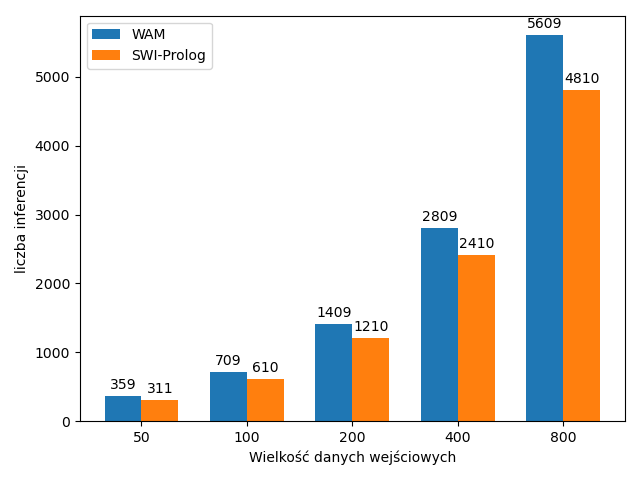
\includegraphics{concati.png}

W przypadku rozcięć liczba inferencji dla proponowanej implementacji i dla SWI-Prologa rośnie liniowo z rozmiarem danych. Dla małych danych SWI-Prolog ma przewagę pod względem liczby inferencji. Przewaga ta też rośnie liniowo.\\

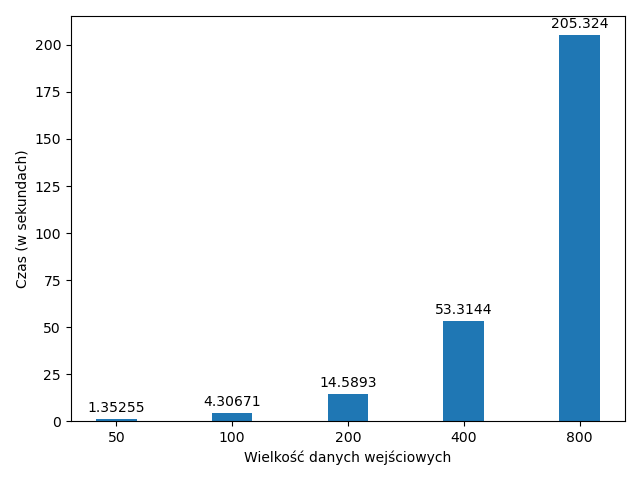
\includegraphics{concattw.png}
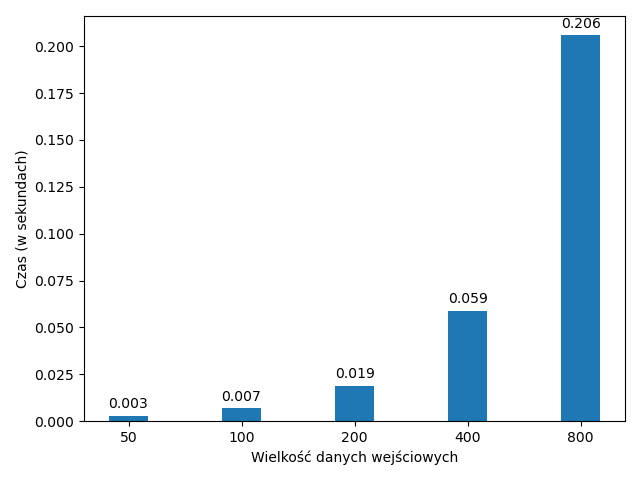
\includegraphics{concatts.png}

Dla pomiarów czasu widać wzrost bliższy kwadratowemu dla obu implementacji, przy czym SWI-Prolog jest około 1000 razy szybszy.

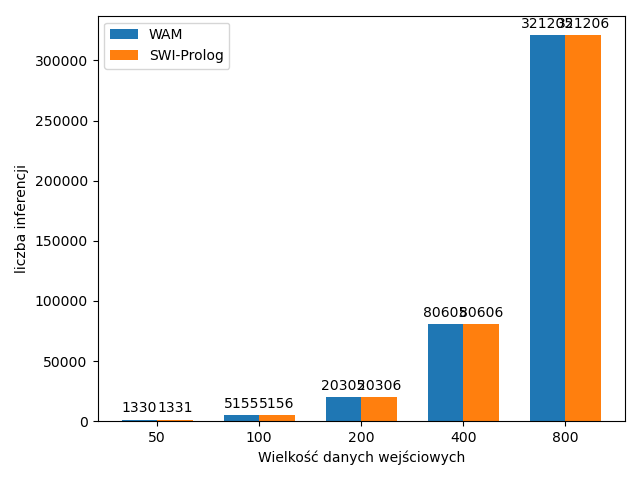
\includegraphics{nrevi.png}

W przypadku naiwenego odwrócenia listy dla dowolnych danych zaproponowana implementacja potrzebuje dokładnie jedną inferencję mniej.

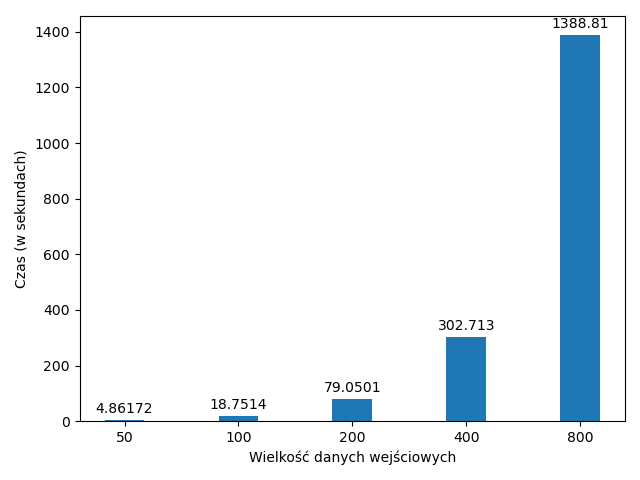
\includegraphics{nrevtw.png}
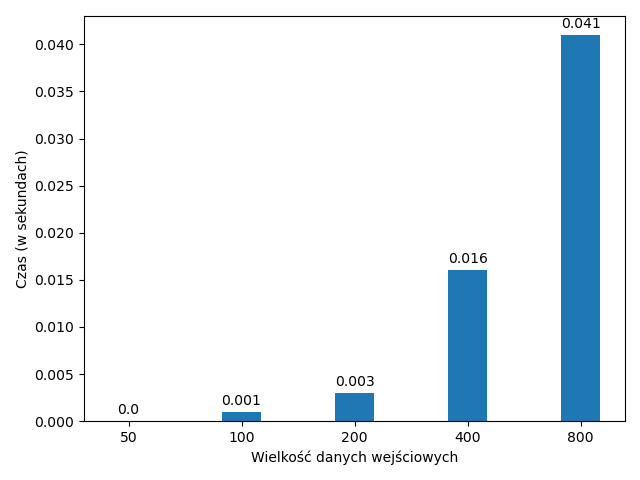
\includegraphics{nrevts.png}

W kategorii czasu dla proponowanej implementacji widać kwadratowy wzrost, to dla SWI-Prologa tempo wzrostu jest trochę mniejsze. SWI-Prolog jest do 33000 razy szybszy.

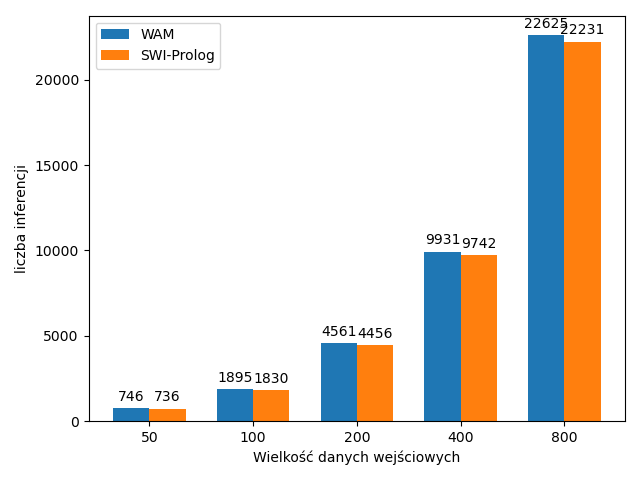
\includegraphics{qsorti.png}

Dla quicksorta różnica w liczbie inferencji tak samo jak dla rozcięć jest na początku niewielka i rośnie ze wzrostem wielkości danych.

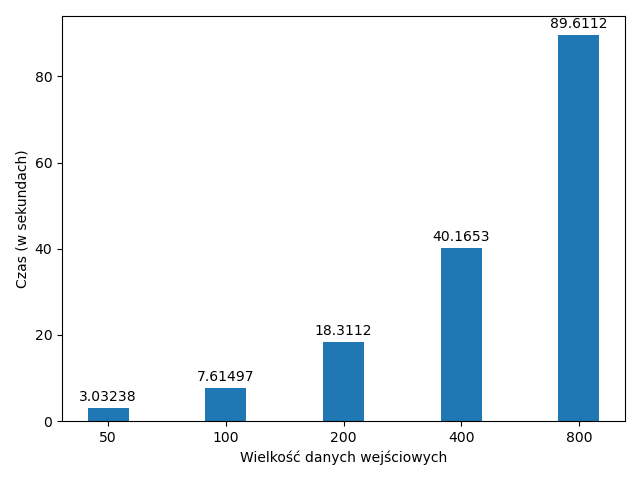
\includegraphics{qsorttw.png}
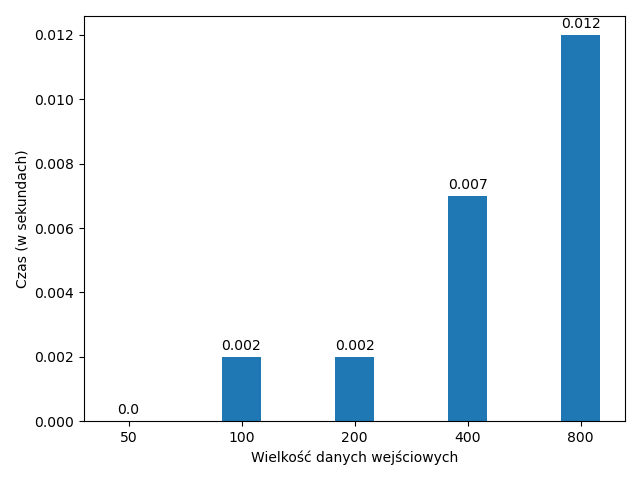
\includegraphics{qsortts.png}

Zależność czasu od wielkości danych jest $O(n\log n)$. SWI-Prolog jest do 7000 razy szybszy.

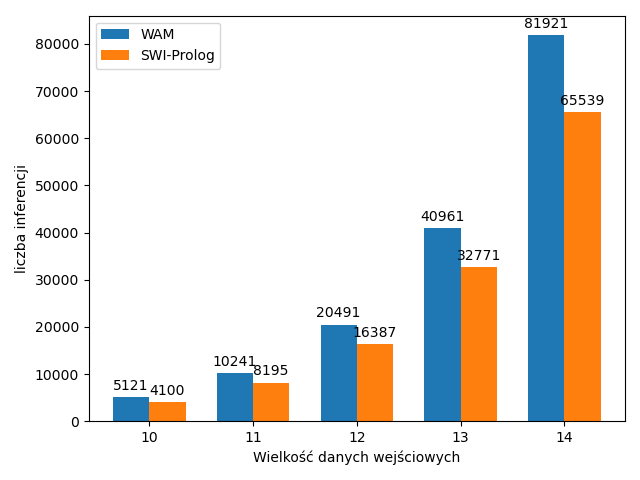
\includegraphics{subsi.png}

W tym wypdaku różnica w liczbie inferencji jest bardziej wyraźna i rośnie wykładniczo.

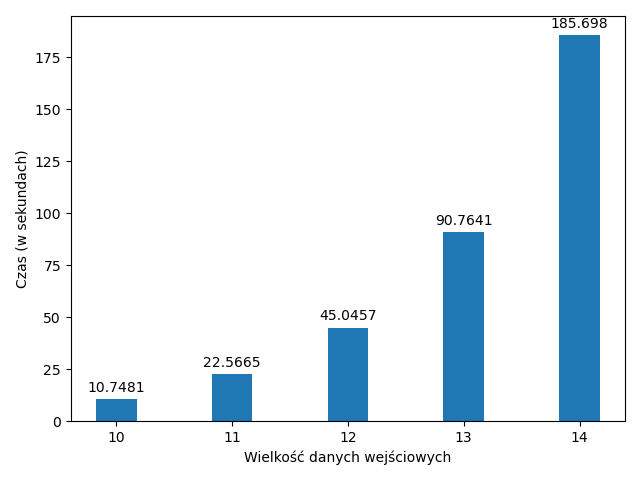
\includegraphics{substw.png}
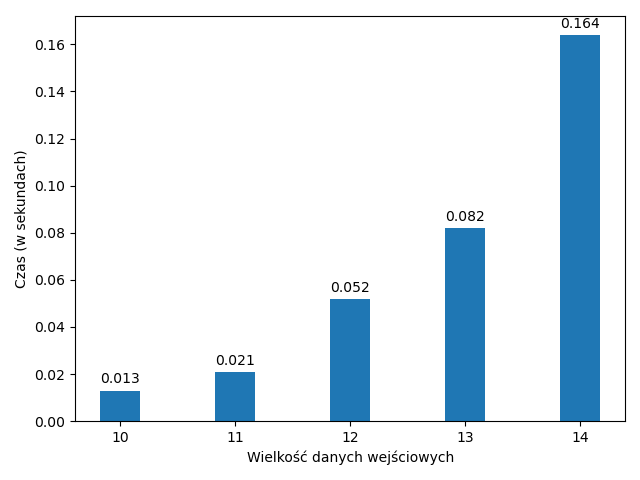
\includegraphics{substs.png}

Potrzebny czas rośnie wykładniczo, a SWI-Prolog jest około 1000 razy szybszy.


	\cleardoublepage

	\chapter{Porównanie z inną implementacją i analiza efektywności}
\thispagestyle{chapterBeginStyle}

\iffalse
W tym rozdziale należy przedstawić analizę zagadnienia, które podlega informatyzacji. Należy zidentyfikować i opisać obiekty składowe rozważanego wycinka rzeczywistości i ich wzajemne relacje (np.\ użytkowników systemu i ich role). Należy szczegółowo omówić procesy jakie zachodzą w systemie i które będą informatyzowane, takie jak np.\ przepływ dokumentów.
Należy sprecyzować i wypunktować założenia funkcjonalne i poza funkcjonalne dla projektowanego systemu.
Jeśli istnieją aplikacje realizujące dowolny podzbiór zadanych funkcjonalności realizowanego systemu należy przeprowadzić ich analizę porównawczą, wskazując na różnice bądź innowacyjne elementy, które projektowany w pracy system informatyczny będzie zawierał.
Należy odnieść się do uwarunkowań prawnych związanych z procesami przetwarzania danych w projektowanym systemie.
Jeśli zachodzi konieczność, należy wprowadzić i omówić model matematyczny elementów systemu na odpowiednim poziomie abstrakcji.

{\color{dgray}
W niniejszym rozdziale omówiono koncepcję architektury programowej systemu \ldots. W
szczególny sposób \ldots. Omówiono założenia funkcjonalne i niefunkcjonalne podsystemów \ldots. Przedstawiono
mechanizmy \ldots. Sklasyfikowano systemy ze względu na \ldots. Omówiono istniejące rozwiązania informatyczne o podobnej funkcjonalności \ldots (zobacz \cite{JCINodesChord}).
}
\fi

W tym rozdziale wymienię kilka istniejących już implementacji Prologa (które zawierają WAM) i porównam szybkość działania jednej z nich z moją implementacją na wybranych testach.\\
3 z popularnych istniejących już implementacji Prologa to:\\
SWI-Prolog - dostępny od 1987 jest prawdopodobnie najpopularniejszą i najbogatszą w dodatkową funkcjonalność implementacją. Jest dostępny na Windowsa, Linuxa i Mac OS X.\\
GNU Prolog - dostępny od 1996 na Windowsa, Linuxa i Mac OS X.\\
YAP Prolog - dostępny od 1985 na Windowsa, Linuxa i Mac OS X. Jest to open-source'owa i działająca wyjątkowo szybko implementacja.\\
W tych implementacjach kompilator i WAM są połączone w jednej aplikacji. W moim rozwiązaniu są to 2 osobne aplikacje (co może ulegnąć zmianie).
	\cleardoublepage
	
	\chapter{Podsumowanie}
\thispagestyle{chapterBeginStyle}

\iffalse
W podsumowanie należy określić stan zakończonych prac projektowych i implementacyjnych. Zaznaczyć, które z zakładanych funkcjonalności systemu udało się zrealizować. Omówić aspekty pielęgnacji systemu w środowisku wdrożeniowym. Wskazać dalsze możliwe kierunki rozwoju systemu, np.\ dodawanie nowych komponentów realizujących nowe funkcje.

W podsumowaniu należy podkreślić nowatorskie rozwiązania zastosowane w projekcie i implementacji (niebanalne algorytmy, nowe technologie, itp.).
\fi

TODO

	\cleardoublepage
	
	
	%%%%%%%%%%%%%%%%%%%%%%%%%%%%%%%%%%%%%%%%%%%%%%%%%%%%%%%%%%%%%%%%%%%%%%%%%%%%%%
	%%%%%%%%%%%%%%%%%%%%%%%%%%%%%%% BIBLIOGRAFIA %%%%%%%%%%%%%%%%%%%%%%%%%%%%%%%%%
	%%%%%%%%%%%%%%%%%%%%%%%%%%%%%%%%%%%%%%%%%%%%%%%%%%%%%%%%%%%%%%%%%%%%%%%%%%%%%%
	
	\pagestyle{bibliographyStyle}
	\bibliographystyle{plabbrv}
	\bibliography{literatura}
	\thispagestyle{chapterBeginStyle}
        \addcontentsline{toc}{chapter}{Bibliografia}

	\cleardoublepage
	
	%%%%%%%%%%%%%%%%%%%%%%%%%%%%%%%%%%%%%%%%%%%%%%%%%%%%%%%%%%%%%%%%%%%%%%%%%%%%%%
	%%%%%%%%%%%%%%%%%%%%%%%%%%%%%%%%% DODATKI %%%%%%%%%%%%%%%%%%%%%%%%%%%%%%%%%%%%
	%%%%%%%%%%%%%%%%%%%%%%%%%%%%%%%%%%%%%%%%%%%%%%%%%%%%%%%%%%%%%%%%%%%%%%%%%%%%%%
	
	\appendix
	\pagestyle{appendixStyle}
	
	\chapter{Zawartość płyty CD}
\thispagestyle{chapterBeginStyle}
\label{plytaCD}

W tym rozdziale należy krótko omówić zawartość dołączonej płyty CD.


	\cleardoublepage

\end{document}

